% Main file: compile this one. Each part of the paper lives in its own file and is pulled in with \input,
% so editing a file under sections/ or appendix/ changes the paper directly.
\documentclass[11pt]{article}
\usepackage[margin=1in]{geometry}
\usepackage{graphicx} % Required for inserting images
\usepackage{amsmath,amssymb,amsthm}
\usepackage{booktabs}
\usepackage{array}
\usepackage{pgfplots}
\pgfplotsset{compat=1.17}
\usepackage[hidelinks]{hyperref}

\newtheorem{theorem}{Theorem}[section]
\newtheorem{proposition}[theorem]{Proposition}
\newtheorem{lemma}[theorem]{Lemma}
\newtheorem{conjecture}[theorem]{Conjecture}
\theoremstyle{definition}
\newtheorem{definition}[theorem]{Definition}
\newtheorem{example}[theorem]{Example}
\theoremstyle{remark}
\newtheorem{remark}[theorem]{Remark}

\newcommand{\F}{F}
\newcommand{\nc}[1]{\langle\!\langle #1 \rangle\!\rangle}
\newcommand{\pres}[2]{\langle #1 \mid #2 \rangle}
\newcommand{\Aut}{\operatorname{Aut}}
\newcommand{\rot}{\operatorname{rot}}
\newcommand{\Sol}{\mathcal{S}}
\newcommand{\Orc}{\mathcal{O}}
\newcommand{\Fix}{\mathcal{F}}
\newcommand{\W}{\mathcal{W}}
\newcommand{\MS}{\mathrm{MS}}
\newcommand{\SMK}{\mathrm{S20\_MK2}}


\title{Stable AC-personal}
\author{Avigya Paudel}
\date{October 2026}

\begin{document}

\maketitle

\paragraph{Notation.} Let $X=\{x_1,\dots,x_n\}$ and let $\F(X)$ be the free group on $X$. A word over
$X^{\pm1}$ is \emph{freely reduced} if it contains no factor $aa^{-1}$ with $a\in X^{\pm1}$, and \emph{cyclically
reduced} if every cyclic permutation of it is freely reduced; a cyclically reduced
word is in particular freely reduced. For $w\in \F(X)$, $|w|$ denotes the length of its freely reduced form. For two generators we write $x,y$. In tables, an upper-case letter denotes an inverse: \texttt{xxxYYYY}
is $x^3y^{-4}$.

% ---- Section 1: AC algorithms ----
\section{AC algorithms}\label{sec:ac}

% ---------BENCHMARKS---------------

\paragraph{Benchmarks.} Every benchmark below is a list of balanced presentations of the trivial
group, all of rank $2$. An \emph{expansion} is one removal of a state from the search heap. For a
presentation $P$, $g(P)$ is the number of expansions GS-SUB \cite{FTS26} needs to solve $P$, and
$g_S(P)$ is the number of expansions our greedy search with the $\SMK$ priority needs. We write $g$
and $g_S$ for these functions of $P$.

\begin{definition}[MS640]
The Miller--Schupp benchmark of \cite{SMM24} is a list of $1{,}190$ presentations $\MS(n,w)$. \textbf{MS640}
\cite{FTS26} is the sublist of the $640$ presentations with $g(P)\le10^6$. Under $\Aut(\F_2)$, MS640, in particular, has $113$ orbits.
\end{definition}

\begin{definition}[bench60]\label{def:bench60}
\textbf{bench60} is a subset of $60$ presentations of MS640: MS640 is split into $10$ bins of $g$, each $3.37$ times
the one below, and $6$ presentations are taken from every bin, spread over the path length and with as few repeated
$\Aut(\F_2)$-orbits as possible. Appendix~\ref{app:bench60} gives the full rule, the bins and where the rows lie in
MS640.
\end{definition}

\begin{definition}[AC19\_autmin]\label{def:ac19}
\textbf{AC19\_autmin} is the extended AC19 data set of \cite{FTS26} ($156{,}762$ balanced
presentations of the trivial group), reduced to one presentation per $\Aut(\F_2)$-orbit.
It has $72{,}779$ rows.
\end{definition}

A presentation of AC19 is AC-trivial if and only if its automorphic form is, so AC19\_autmin
carries the same AC-triviality questions as AC19. However, an automorphism of a presentation can be much harder or easier to search than the original presentation.

\begin{definition}[ladder100]\label{def:ladder}\label{def:levels}
\textbf{ladder100} has $10$ presentations from AC19\_autmin and MS640 in each of the $10$ levels of Table~\ref{tab:ladder}, graded by $g$; $g>10^7$ means LENGTH fails within $10^7$ expansions, and $g_S$ is the $\SMK$
expansion count. Levels $1$--$6$ spread their rows over the range of $g$ and level $9$ over the range of $g_S$, level $8$ takes the
largest $g$, and level $7$ the largest $g_S$. Level $10$ holds the presentations on which $\SMK$ also fails within $10^7$ expansions. All of these presentations are verified to be AC-trivial by solving their initial automorphic state in $AC19$ extended dataset and using the same S-moves on the aut-min state.

The purpose of creating this new benchmark was to raise the difficulty to even higher levels (up to presentations that are AC trivial but cannot be solved by greedy substitution even with $10^{7}$ nodes). This can help discover new algorithms capable of solving problems closer to the second hump \cite{FTS26}.

\end{definition}

\begin{table}[ht]
\centering
\begin{tabular}{rlrrrr}
\toprule
level & $g$ & from MS640 & mean $\lambda$ & mean $g$ & mean $g_S$\\
\midrule
1 & $<10^3$ & $5$ & $15.3$ & $214$ & $101$\\
2 & $10^3$--$10^4$ & $5$ & $19.9$ & $3{,}983$ & $707$\\
3 & $10^4$--$10^{4.5}$ & $5$ & $21.1$ & $17{,}612$ & $7{,}646$\\
4 & $10^{4.5}$--$10^5$ & $5$ & $21.5$ & $56{,}183$ & $9{,}780$\\
5 & $10^5$--$10^{5.5}$ & $4$ & $22.5$ & $235{,}756$ & $13{,}312$\\
6 & $10^{5.5}$--$10^6$ & $2$ & $19.4$ & $588{,}638$ & $4{,}693$\\
7 & $10^6$--$3\cdot10^6$ & $0$ & $20.2$ & $1{,}875{,}962$ & $424{,}977$\\
8 & $3\cdot10^6$--$10^7$ & $0$ & $18.8$ & $5{,}022{,}975$ & $113{,}309$\\
9 & $>10^7$ & $0$ & $21.0$ & -- & $340{,}650$\\
10$^{*}$ & $>10^7$ & $0$ & $18.3$ & -- & --\\
\bottomrule
\end{tabular}

\smallskip
{\small $^{*}$Only $9$ presentations fail for $\SMK$, so the tenth, \texttt{ac19\_12445}, is the next hardest one for
$\SMK$ from level $9$: it needs $1{,}297{,}772$ expansions.}
\caption{The levels of ladder100: the range of $g$, the number of the $10$ presentations taken from MS640 (the rest
are from AC19\_autmin), and the means of the starting total length $\lambda$, of $g$ and of $g_S$.}
\label{tab:ladder}
\end{table}

\paragraph{Units.} Every budget is counted in \emph{units}. For LENGTH and $\SMK$ (Definitions~\ref{def:greedy}
and~\ref{def:smk}) a unit is one \emph{expansion}: remove the first state from the heap, generate its S-move children,
drop those already discovered and push the rest onto the heap by priority. The CoV used here (Section~\ref{sec:cov}) is
one-shot: it is applied once, to the starting presentation, before any search, and builds new presentations, which
LENGTH then searches. Building them costs no units. For the hybrid (Definition~\ref{def:hybrid}) a unit is one
expansion of its search or one S-move of its finishing checks. A budget is per
presentation, a failed search is charged all of it, and path lengths are counted in S-moves (for the hybrid, S-moves plus Nielsen images).

\paragraph{Time per unit.} A pop does different work in each method: LENGTH and $\SMK$ differ in the priority they
compute, the hybrid also builds Nielsen images and runs finishing checks, and CoV creates images instead of S-move
children. Equal budgets in units are a fair comparison only if a unit costs about the same in each method, so we time
one pop of each method on the same states. On each test state, each method starts a fresh search, so the heap holds
only that state, and makes one pop: it removes the state, creates all its children, discards those already discovered,
computes the priorities of the rest and pushes them onto the heap. The test states are drawn at random from the states
that LENGTH and $\SMK$ popped on MS640 with a budget of $10^4$ units, up to $60$ per range of total length $\lambda$,
and every method is timed on the same states. All run in pure Python (one core, Intel Xeon $2.1$ GHz, best of five
runs).
\begin{center}
\small
\begin{tabular}{lrrrrr}
\toprule
$\lambda$ & states & LENGTH & $\SMK$ & hybrid & CoV\\
\midrule
$\le10$ & $46$ & $0.12$ & $0.14$ & $0.28$ & $0.25$\\
$11$--$15$ & $60$ & $0.85$ & $1.05$ & $1.37$ & $3.24$\\
$16$--$20$ & $60$ & $1.61$ & $2.00$ & $3.03$ & $6.05$\\
$21$--$25$ & $60$ & $2.99$ & $3.41$ & $10.08$ & $11.23$\\
$\ge26$ & $60$ & $4.66$ & $6.00$ & $6.85$ & $16.47$\\
\midrule
mean & & $2.04$ & $2.52$ & $4.32$ & $7.45$\\
relative to LENGTH & & $1$ & $1.23$ & $2.11$ & $3.64$\\
\bottomrule
\end{tabular}

\smallskip
\footnotesize Time of one pop in ms, averaged over the states of the row. The mean row averages the five rows; the last row divides it by the LENGTH mean.
\end{center}
For example, one pop of $\mathrm{AK}(3)$ ($\lambda=13$) takes $0.69$ ms for LENGTH, $0.87$ ms for $\SMK$, $1.17$ ms
for the hybrid and $2.61$ ms for CoV. A longer state has more children, so its pop costs more. An $\SMK$ pop differs
from a LENGTH pop only in its priority and costs $1.1$--$1.3$ times as much. A hybrid pop also builds the four Nielsen
images and runs the finishing checks, and costs $1.5$--$3.4$ times as much; its other units are single moves and cost
less. A CoV pop costs $3.5$--$3.8$ LENGTH pops for $\lambda>10$, but CoV makes it only once, on the starting
presentation, which is why it is not charged. A unit of each method thus costs within a small factor of one LENGTH
expansion, and equal budgets in units are comparable up to that factor.

\subsection{AC search methods}\label{sec:methods}

The three methods below are AC search methods: each solve comes with an AC certificate. All three search over
S-moves; LENGTH and $\SMK$ use nothing else.

\begin{definition}[S-move and state]\label{def:smove}
For a cyclically reduced word $r$ and $0\le k<|r|$, let $\rot_k(r)$ be $r$ with its last $k$ letters moved to the
front. A \emph{substitution move} (S-move) $(i,j,s,k_1,k_2)$, with $i\neq j$, $s=\pm1$ and the last letter of $\rot_{k_1}(r_i)$ inverse to the first letter of
$\rot_{k_2}(r_j^{\,s})$, replaces
\[
r_i\;\longmapsto\;\rot_{k_1}(r_i)\cdot\rot_{k_2}\!\big(r_j^{\,s}\big)
\]
and cyclically reduces \cite{FTS26}. A \emph{state} is a presentation up to rotation and inversion of each relator and permutation of the relators,
stored in a canonical form described in \cite{FTS26}.
\end{definition}

\begin{definition}[Greedy search]\label{def:greedy}
A greedy search with priority $\pi$, budget $B$ and length bound $c$ keeps a heap of states, lowest $\pi$ first,
starting from the input. An \emph{expansion} removes the first state $Q$: if every relator of $Q$ has length $1$, $Q$
is solved; otherwise the children of $Q$ under S-moves that are new and have every relator of length at most $c$ are pushed onto the heap. The search stops after $B$ pops, and the certificate is the chain of parent moves. Ties in $\pi$ are broken by depth and then by a fixed order on states described in \cite{FTS26}, so every run is deterministic.
\end{definition}

The two greedy searches below differ only in the priority, that is, in which state they expand next.

\begin{definition}[LENGTH]\label{def:length}
\emph{LENGTH} is the greedy search with $\pi=\lambda$, the total length: it always expands a shortest state. It is the
greedy search of \cite{SMM24}.
\end{definition}

\begin{definition}[$\SMK$]\label{def:smk}
Read each relator cyclically. A \emph{block} is a maximal run of letters of one generator, $x$ and $x^{-1}$ counted
alike. For a state $Q$:
\begin{itemize}
  \item $\mathrm{MK}(Q)$ is the largest number of $x$-blocks or of $y$-blocks in a single relator of $Q$ (a relator
  that is a power of one generator counts $0$);
  \item $S(Q)$ is the mean length of the $x$-blocks or of the $y$-blocks, pooled over both relators, whichever is
  smaller (a generator that does not occur is ignored).
\end{itemize}
$\SMK$ is the greedy search with
\[
\pi_{\SMK}(Q)=\lambda(Q)+20\,S(Q)+2\,\mathrm{MK}(Q).
\]
\end{definition}

\begin{example}
Take $\mathrm{AK}(3)=\pres{x,y}{x^3y^{-4},\ xyxy^{-1}x^{-1}y^{-1}}$. The first relator has the blocks
$x^3\mid y^{-4}$, one of each generator; the second has the six blocks $x\mid y\mid x\mid y^{-1}\mid x^{-1}\mid y^{-1}$,
three of each. Hence $\mathrm{MK}=3$. The $x$-blocks have lengths $3,1,1,1$, mean $1.5$, and the $y$-blocks
$4,1,1,1$, mean $1.75$, so $S=1.5$. With $\lambda=13$,
\[
\pi_{\SMK}(\mathrm{AK}(3))=13+20\cdot1.5+2\cdot3=49,\qquad \pi_{\mathrm{LENGTH}}(\mathrm{AK}(3))=13.
\]
\end{example}

\begin{remark}[Choice of $S$ and $\mathrm{MK}$]
The features $S$ and $\mathrm{MK}$ come from comparing, on the starting presentations of MS1190, the $640$ rows that
LENGTH solves with the $550$ it does not, and keeping the features that best separate the two groups. They are
imperfect: no feature of a single state can decide whether a presentation is easy or hard. For example,
\[
\pres{x,y}{y^{-1}x^{-1}yxy^{-1}x,\ y^{-4}x^3}
\qquad\text{and}\qquad
\pres{x,y}{y^{-1}x^{-1}y^{-1}xyx,\ y^{-4}x^3}
\]
have the same $\lambda=13$, $\mathrm{MK}=3$ and $S=1.5$, hence the same $\pi_{\SMK}=49$. LENGTH solves the first in
$107$ expansions, with a path of $19$ S-moves, while the second is $\mathrm{AK}(3)$. For example, length is also an imperfect heuristic, but the idea here is to obtain features that represent a state that might be easier to solve on average so that temporarily increasing the length can be a possibility.
\end{remark}

\begin{definition}[Hybrid solver]\label{def:hybrid}
The input is a balanced presentation $P$ of rank $2$ with $|\det M|=1$, where $M$ is the $2\times2$ matrix of exponent
sums of the relators, and the \emph{Nielsen maps} are
$x\mapsto xy^{\pm1}$ and $y\mapsto yx^{\pm1}$. The solver has two parts (Figure~\ref{fig:hybrid}).
\begin{enumerate}
  \item \emph{Finishing checks.} Two shapes are finished directly by S-moves. (i) A generator occurs once in a relator
  (Proposition~\ref{prop:once}). (ii) A relator
  reads cyclically as $g^ah^pg^{-a}h^q$ and its pinch replacements bring the other relator to at most one $g$-block
  (Proposition~\ref{prop:pinch}).
  \item \emph{Search.} If the checks do not finish $P$, a best-first search with priority $\lambda$, on states taken
  up to signed permutations of the generators. The children of a state are its S-move children and its four Nielsen images. Every new child goes through two filters that change nothing
  (Definition~\ref{def:filters}); a child that passes goes to the check they name, which then finishes it
  (Proposition~\ref{prop:filters}). The other children are pushed onto the heap.
\end{enumerate}
The \emph{units} of a run are its pops, plus one for every S-move that a check applies.
\end{definition}

\begin{figure}[ht]
\centering
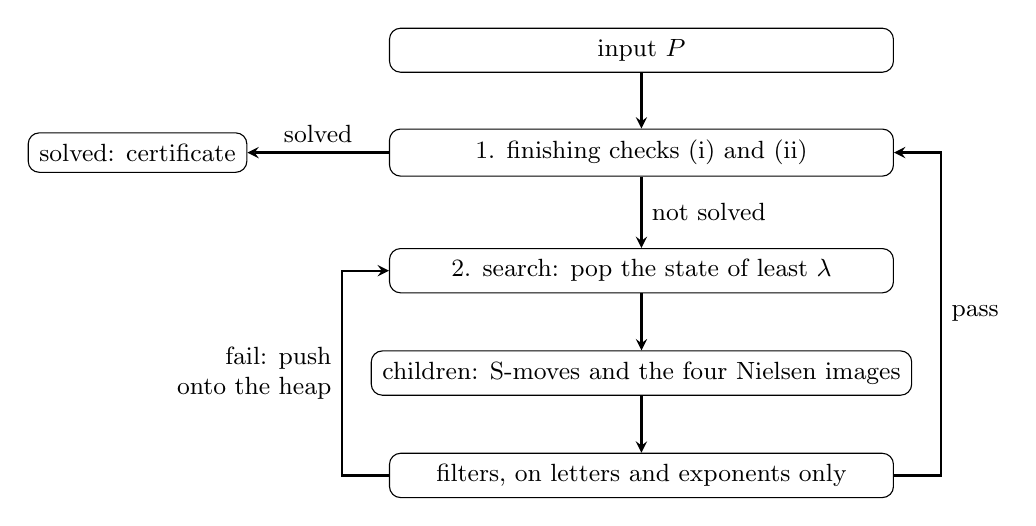
\begin{tikzpicture}[x=1cm,y=1cm,font=\small,
  box/.style={draw,rounded corners,align=center,inner sep=4pt,minimum width=6.4cm},
  arr/.style={->,>=stealth,thick}]
  \node[box] (in) at (0,0) {input $P$};
  \node[box] (fin) at (0,-1.3) {1. finishing checks (i) and (ii)};
  \node[draw,rounded corners,inner sep=4pt] (out) at (-6.4,-1.3) {solved: certificate};
  \node[box] (pop) at (0,-2.8) {2. search: pop the state of least $\lambda$};
  \node[box] (kids) at (0,-4.1) {children: S-moves and the four Nielsen images};
  \node[box] (filt) at (0,-5.4) {filters, on letters and exponents only};
  \draw[arr] (in) -- (fin);
  \draw[arr] (fin.west) -- node[above]{solved} (out);
  \draw[arr] (fin) -- node[right]{not solved} (pop);
  \draw[arr] (pop) -- (kids);
  \draw[arr] (kids) -- (filt);
  \draw[arr] (filt.west) -- ++(-0.6,0) |- node[pos=0.25,left,align=right]{fail: push\\onto the heap} (pop.west);
  \draw[arr] (filt.east) -- ++(0.6,0) |- node[pos=0.25,right,align=left]{pass} (fin.east);
\end{tikzpicture}
\caption{The hybrid solver. A child that passes the filters goes to the finishing checks, which then finish it; the
other children are pushed onto the heap.}
\label{fig:hybrid}
\end{figure}

The hybrid stays at rank $2$, so its certificates are AC paths. It can also change the rank during the search
(Section~\ref{sec:hybrid}); that extension is left out here.

\paragraph{Scores.} We compare the three methods at equal budgets in units: the number of
presentations each solves on the three benchmarks.

\begin{center}
\small
\begin{tabular}{llrrrrr}
\toprule
& & \multicolumn{5}{c}{budget (units)}\\
\cmidrule(lr){3-7}
benchmark & method & $10^3$ & $10^4$ & $10^5$ & $10^6$ & $10^7$\\
\midrule
MS640 & LENGTH & $554$ & $606$ & $634$ & $640$ & $640$\\
(of $640$) & $\SMK$ & $574$ & $626$ & $640$ & $640$ & $640$\\
& dual, single CoV & $593$ & $621$ & $640$ & $640$ & $640$\\
& dual, auto CoV & $614$ & $634$ & $640$ & $640$ & $640$\\
& triple$^{\dagger}$ & $612$ & $634$ & $640$ & $640$ & $640$\\
& hybrid & $640$ & $640$ & $640$ & $640$ & $640$\\
\midrule
bench60 & LENGTH & $29$ & $40$ & $54$ & $60$ & $60$\\
(of $60$) & $\SMK$ & $37$ & $52$ & $60$ & $60$ & $60$\\
& dual, single CoV & $43$ & $52$ & $60$ & $60$ & $60$\\
& dual, auto CoV & $51$ & $56$ & $60$ & $60$ & $60$\\
& triple$^{\dagger}$ & $49$ & $56$ & $60$ & $60$ & $60$\\
& hybrid & $60$ & $60$ & $60$ & $60$ & $60$\\
\midrule
ladder100 & LENGTH & $11$ & $20$ & $40$ & $60$ & $80$\\
(of $100$) & $\SMK$ & $23$ & $53$ & $69$ & $87$ & $91$\\
& dual, single CoV & $56$ & $82$ & $100$ & $100$ & $100$\\
& dual, auto CoV & $77$ & $96$ & $100$ & $100$ & $100$\\
& triple$^{\dagger}$ & $81$ & $97$ & $100$ & $100$ & $100$\\
& hybrid & $99$ & $100$ & $100$ & $100$ & $100$\\
\bottomrule
\end{tabular}

\smallskip
\footnotesize Dual and triple: the greedy searches of ACSolverES (E.~Steffen), with the CoV work counted in
substitution-pop units. Counted in nodes, where a CoV pop counts as $1$, the $10^3$ / $10^4$ columns read: single CoV
$604$/$627$, $46$/$52$, $64$/$92$; auto CoV $618$/$634$, $51$/$56$, $80$/$97$; triple $618$/$634$, $51$/$56$,
$86$/$97$. Every row is solved within $10^5$, so the $10^6$ and $10^7$ columns are full.
$^{\dagger}$The triple's complete CoV is not an automorphism, so $54$, $7$ and $17$ of its solves prove only stable
AC-triviality.
\end{center}

$\SMK$ solves all of MS640 and bench60 by $10^5$ units, LENGTH only by $10^6$. On ladder100 neither finishes by
$10^7$: $9$ rows are unsolved by both. The hybrid solves all of MS640 and bench60 at $10^3$ units and all of
ladder100 at $10^4$; its hardest row, \texttt{ac19\_70845}, takes $2{,}267$ units.

\paragraph{Units and path lengths.} For every solve we also record the units it took and the length of its path:
S-moves, and for the hybrid S-moves plus Nielsen images.

\begin{center}
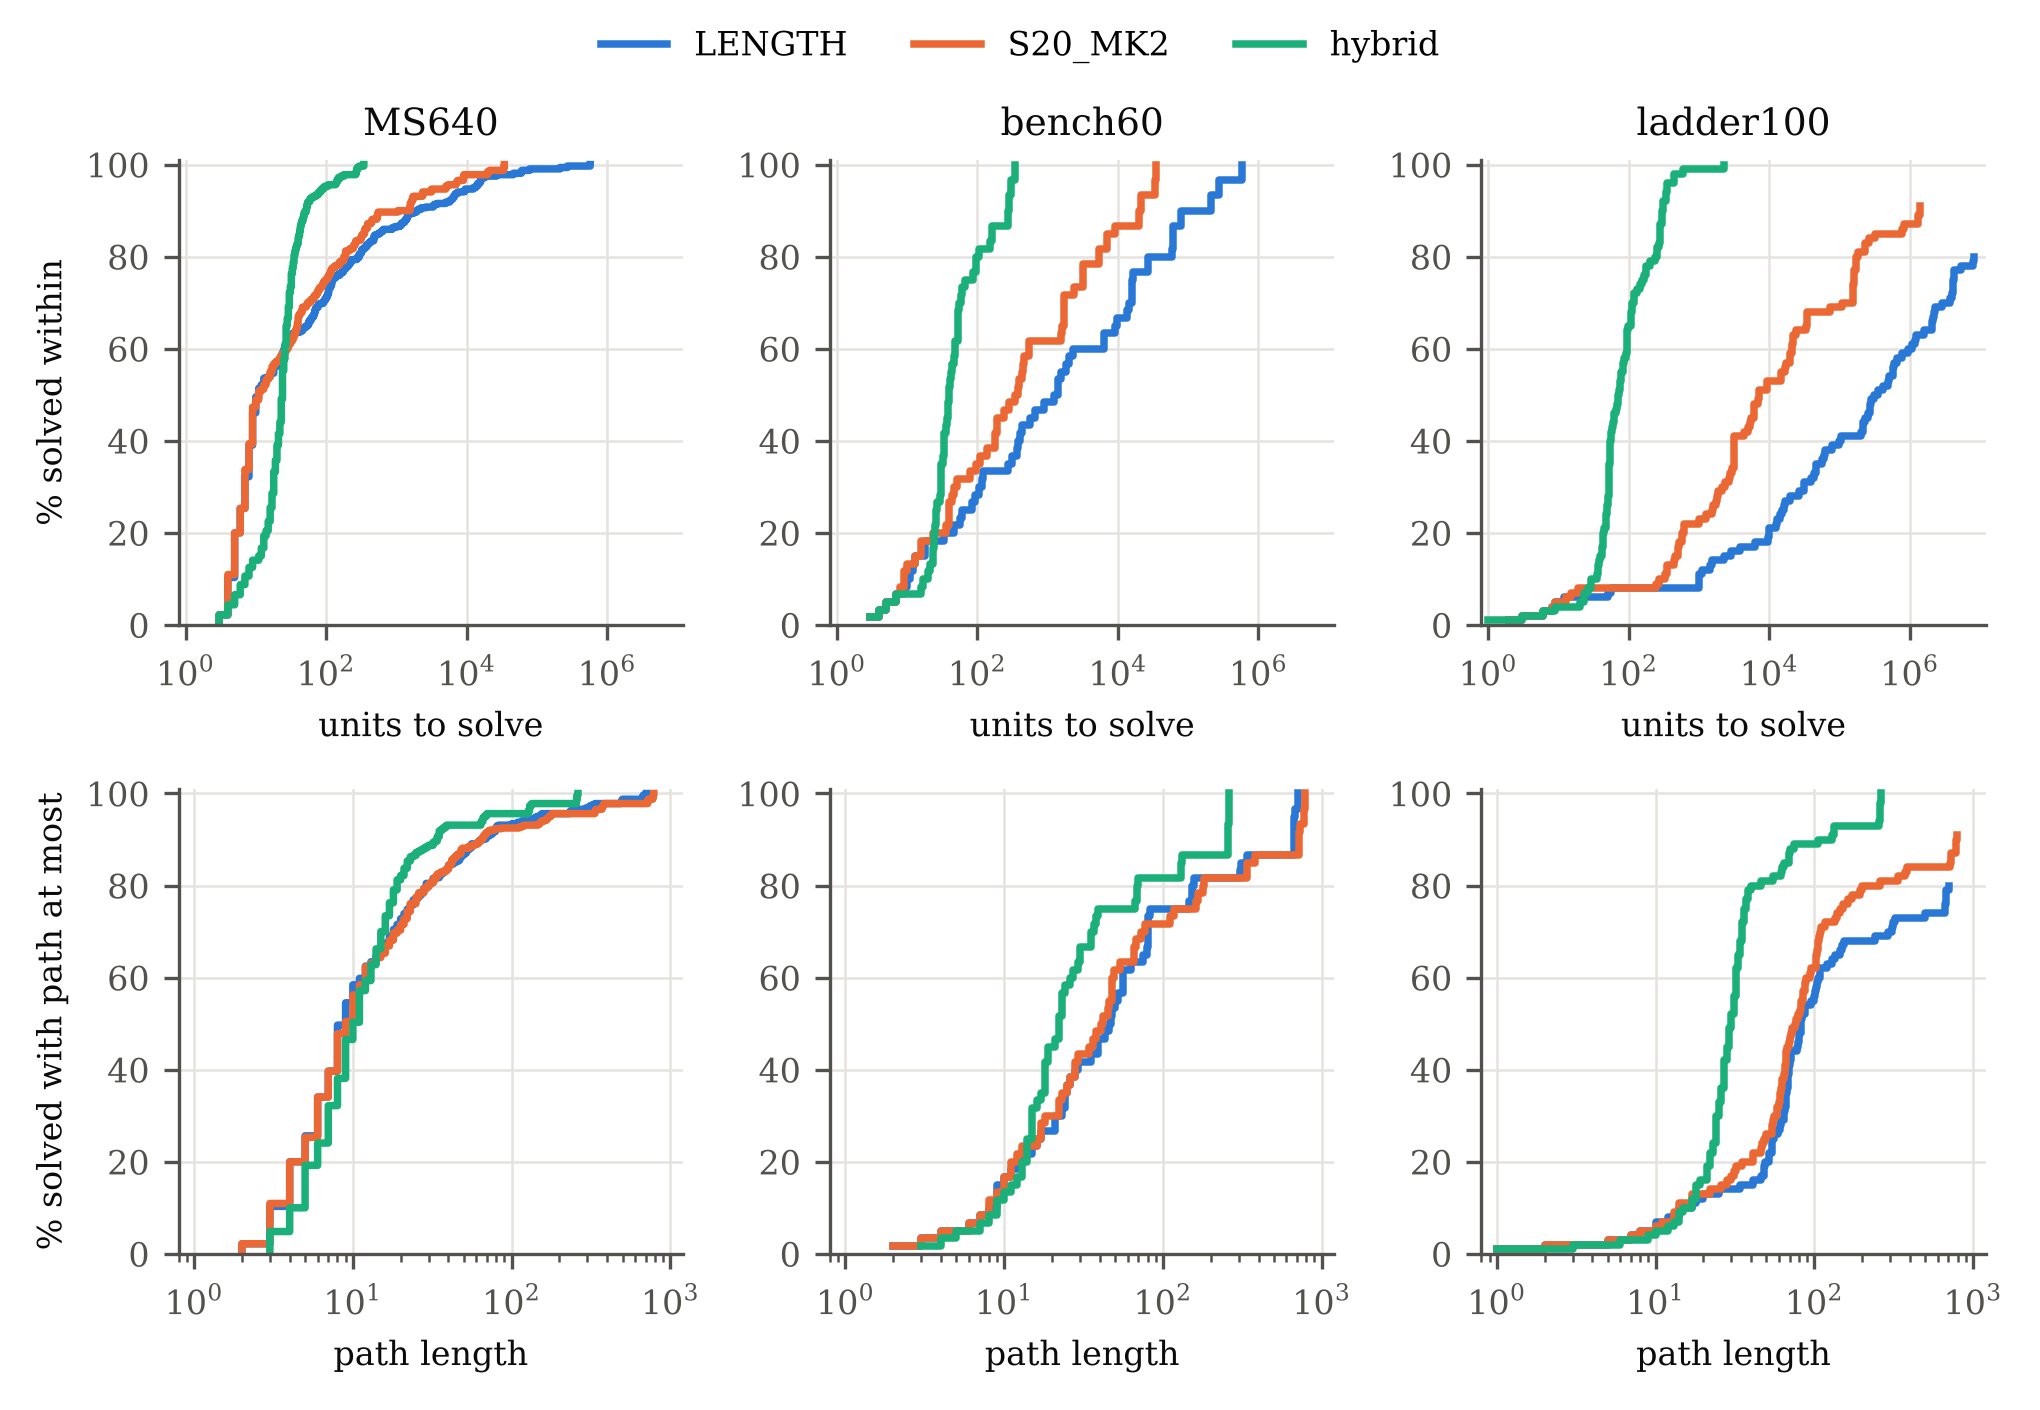
\includegraphics[width=\textwidth]{figures/units_paths.png}
\end{center}

\begin{center}
\small
\begin{tabular}{llrrrrrr}
\toprule
& & \multicolumn{3}{c}{units to solve} & \multicolumn{3}{c}{path length}\\
\cmidrule(lr){3-5}\cmidrule(lr){6-8}
benchmark & method & mean & median & max & mean & median & max\\
\midrule
MS640 & LENGTH & $4{,}963$ & $11$ & $574{,}959$ & $36.8$ & $9$ & $708$\\
 & $\SMK$ & $995$ & $11$ & $34{,}438$ & $42.9$ & $9$ & $787$\\
 & dual, single CoV & $729$ & $31$ & $25{,}854$ & $40.8$ & $10$ & $825$\\
 & dual, auto CoV & $349$ & $14$ & $18{,}110$ & $44.0$ & $9$ & $939$\\
 & triple$^{\dagger}$ & $376$ & $22$ & $18{,}745$ & $44.1$ & $9$ & $939$\\
 & hybrid & $23$ & $11$ & $322$ & $21.2$ & $10$ & $262$\\
\midrule
bench60 & LENGTH & $45{,}244$ & $1{,}311$ & $574{,}959$ & $142.6$ & $47$ & $708$\\
 & $\SMK$ & $4{,}685$ & $359$ & $34{,}438$ & $154.3$ & $42$ & $787$\\
 & dual, single CoV & $3{,}509$ & $326$ & $25{,}582$ & $148.0$ & $45$ & $780$\\
 & dual, auto CoV & $1{,}795$ & $192$ & $18{,}079$ & $161.8$ & $39$ & $939$\\
 & triple$^{\dagger}$ & $1{,}879$ & $198$ & $18{,}637$ & $161.7$ & $39$ & $939$\\
 & hybrid & $67$ & $28$ & $322$ & $59.9$ & $22$ & $262$\\
\midrule
ladder100 & LENGTH & $975{,}165$ & $101{,}771$ & $8{,}204{,}360$ & $130.8$ & $69$ & $706$\\
 & $\SMK$ & $114{,}830$ & $6{,}073$ & $1{,}383{,}279$ & $133.9$ & $69$ & $787$\\
 & dual, single CoV & $4{,}654$ & $796$ & $61{,}821$ & $114.7$ & $58$ & $780$\\
 & dual, auto CoV & $1{,}523$ & $315$ & $18{,}113$ & $122.2$ & $58$ & $939$\\
 & triple$^{\dagger}$ & $1{,}373$ & $314$ & $18{,}680$ & $121.2$ & $54$ & $939$\\
 & hybrid & $127$ & $53$ & $2{,}267$ & $49.7$ & $30$ & $262$\\
\bottomrule
\end{tabular}

\smallskip
\footnotesize Over the rows each method solves (on ladder100: $80$, $91$, all $100$ for the dual and triple
searches, and $100$). Dual and triple: units count the CoV work in substitution-pop units, and a path counts each CoV
move as one step (a map $x\mapsto xy^k$ counts $1$). $^{\dagger}$Stable AC certificate on $54$, $7$ and $17$ of the
rows.
\end{center}


On easy rows the hybrid spends about as many units as the greedy searches (median $11$ against $11$ on MS640); on
hard rows it needs far fewer, at most $2{,}267$ against $8.2$ million for LENGTH.
Its paths are shorter on hard rows too: on the $80$ ladder100 rows that all three solve, $53.8$ steps on average
against $130.8$ for LENGTH and $142.4$ for $\SMK$. $\SMK$ paths are about as long as LENGTH's.

\subsection{Pinch replacements}\label{sec:pinch}

Below, $P=\pres{x,y}{r,s}$ with $|\det M|=1$ and $\{g,h\}=\{x,y\}$. S-moves and Nielsen maps preserve $|\det M|$, so
every state of the search has $|\det M|=1$. A relator splits into \emph{blocks} (Definition~\ref{def:smk}):
$x^2y^{-1}x^{-3}y$ has the four blocks $x^2\mid y^{-1}\mid x^{-3}\mid y$. A relator $r$ is a \emph{pinch form} if it
reads cyclically as $g^ah^pg^{-a}h^q$ with $a>0$ and $p,q\neq0$; it says $g^ah^pg^{-a}=h^{-q}$ and
$g^{-a}h^qg^a=h^{-p}$.

\begin{lemma}[Pinch replacements]\label{lem:pinch}
Let $r=g^ah^pg^{-a}h^q$ be a pinch form and $n\in\mathbb Z$. If $s$, read cyclically, contains $g^ah^{np}g^{-a}$, then
$|n|$ S-moves by $r^{\pm1}$ replace it by $h^{-nq}$. Likewise $|n|$ S-moves replace $g^{-a}h^{nq}g^a$ by $h^{-np}$.
\end{lemma}

\begin{proof}
Let $n>0$. Rotate $s$ to $v\,g^ah^p$, ending with the first $g^ah^p$ of the occurrence, and multiply by
$h^{-p}g^{-a}h^{-q}g^a$, a rotation of $r^{-1}$. The seam cancels, so this is an S-move, and
\[
v\,g^ah^p\cdot h^{-p}g^{-a}h^{-q}g^a=v\,h^{-q}g^a .
\]
So $g^a$ moves one step right and turns $h^p$ into $h^{-q}$. After $n$ moves $g^ah^{np}$ is $h^{-nq}g^a$, and
$g^ag^{-a}$ cancels. For $n<0$ the factor is $h^pg^{-a}h^qg^a$, a rotation of $r$. The second replacement uses
$h^{-q}g^ah^{-p}g^{-a}=r^{-1}$, or $h^qg^ah^pg^{-a}$ for $n<0$.
\end{proof}

\begin{example}\label{ex:replace}
Let $s=g^ah^{3p}g^{-a}w$, with $w$ any word. Each step replaces the first $g^ah^p$ by $h^{-q}g^a$, one S-move as in
the proof:
\begin{align*}
s&=g^ah^p\cdot h^{2p}g^{-a}w &&(h^{3p}\text{ to pass})\\
&\to h^{-q}g^ah^p\cdot h^{p}g^{-a}w &&(h^{2p}\text{ left})\\
&\to h^{-2q}g^ah^p\cdot g^{-a}w &&(h^{p}\text{ left})\\
&\to h^{-3q}g^ag^{-a}w=h^{-3q}w.
\end{align*}
In full, the first step rotates $s$, multiplies by $h^{-p}g^{-a}h^{-q}g^a$, and rotates back ($\sim$ is rotation):
\[
s\sim h^{2p}g^{-a}w\cdot g^ah^p\;\to\;h^{2p}g^{-a}w\cdot g^ah^p\cdot h^{-p}g^{-a}h^{-q}g^a=h^{2p}g^{-a}w\,h^{-q}g^a
\sim h^{-q}g^ah^{2p}g^{-a}w.
\]
Three S-moves replace $g^ah^{3p}g^{-a}$ by $h^{-3q}$, and the $g^a$ and $g^{-a}$ are gone.
\end{example}

\paragraph{Check (ii).} Let $r=g^ah^pg^{-a}h^q$ be a pinch form. Check (ii) uses Lemma~\ref{lem:pinch} on the other
relator $s$ again and again: while $s$ contains $g^ah^{np}g^{-a}$ or $g^{-a}h^{nq}g^a$, replace it by $h^{-nq}$ or
$h^{-np}$. Each replacement removes $2a$ letters $g$, so this stops, either with at most one $g$-block left in $s$, or
with neither factor in $s$. Which of the two happens depends only on the exponents of the blocks of $s$, so the check
first works it out on these integers, without moves. If $s$ ends with at most one $g$-block, the replacements are
made as S-moves and Proposition~\ref{prop:pinch} finishes $P$. Otherwise no move is made and the state is pushed onto
the heap. Both relators are tried as $r$.

\subsection{Filters}

\begin{definition}[Filters]\label{def:filters}
A state $Q=(r,s)$ passes
\begin{enumerate}
  \item[(F1)] if a relator has a generator occurring once or has exactly four blocks;
  \item[(F2)] if a relator has a generator occurring once (check (i)), or a relator is a pinch form whose
  replacements, worked out on the exponents, bring the other relator to at most one $g$-block (check (ii)).
\end{enumerate}
\end{definition}

A child is tested by (F1), then by (F2) if it passed (F1), then finished by its check if it passed (F2); every other
child is pushed onto the heap. (F1) counts letters and blocks, about $1\,\mu$s per child; (F2) is integer arithmetic
on the exponents. Neither makes a move or costs units.

\subsection{Finishing checks}

\begin{proposition}[Check (i), one occurrence]\label{prop:once}
If $g$ occurs exactly once in $r$, then $P$ is AC-trivial, by at most $n_g(s)+|k|$ S-moves, where $r=gh^k$ up to
rotation and inversion and $n_g(s)$ is the number of letters $g^{\pm1}$ in $s$.
\end{proposition}

\begin{proof}
While $g$ occurs in $s$, rotate $s$ to $ug^{\varepsilon}$ and multiply by the rotation of $r^{-\varepsilon}$ that begins
with $g^{-\varepsilon}$: one S-move, giving $uh^{-\varepsilon k}$. After at most $n_g(s)$ moves $s=h^m$. The rows of
$M$ are $(1,k)$ and $(0,m)$, so $|m|=1$. Then $|k|$ S-moves by $s^{\pm1}$ delete the $h$'s of $r$, leaving
$(g,h^{\pm1})$, which is $T_2=\pres{x,y}{x,y}$ up to inversion.
\end{proof}

\begin{proposition}[Check (ii), pinch]\label{prop:pinch}
If $r$ is a pinch form and its replacements bring $s$ to at most one $g$-block, then $P$ is AC-trivial.
\end{proposition}

\begin{proof}
By Lemma~\ref{lem:pinch} the replacements are S-moves; they give $(r,s')$ with $s'$ having at most one $g$-block
$g^e$, and $|\det M|=1$. The exponent sums are $(0,p+q)$ for $r$ and $(e,m)$ for $s'$, so $|e|\,|p+q|=1$ and $|e|=1$:
$g$ occurs once in $s'$, and Proposition~\ref{prop:once} finishes.
\end{proof}

\begin{proposition}\label{prop:filters}
A child passes (F2) if and only if check (i) or (ii) finishes it, and every child that passes (F2) passes (F1).
\end{proposition}

\begin{proof}
(F2) holds exactly when check (i) or (ii) applies, and then Proposition~\ref{prop:once} or~\ref{prop:pinch} finishes
the child. A pinch form has exactly four blocks, so (F2) implies (F1).
\end{proof}


% ---- Section 2: stable AC algorithms ----
\section{Stable AC algorithms}\label{sec:stable}

\begin{definition}[Stable AC moves]\label{def:stableac}
The \emph{AC moves} on $\pres{X}{r_1,\dots,r_n}$ are (AC1) $r_i\mapsto r_ir_j$ for $i\neq j$, (AC2) $r_i\mapsto
r_i^{-1}$ and (AC3) $r_i\mapsto gr_ig^{-1}$ for $g\in X^{\pm1}$. The \emph{trivial presentation} is $\pres{X}{X}$.
The \emph{stable AC moves} add two more, for a generator $z\notin X$:
\begin{align*}
&(\mathrm{AC4})\quad \pres{X}{R}\ \longmapsto\ \pres{X,z}{R,\,z},\\
&(\mathrm{AC5})\quad \pres{X,z}{R,\,z}\ \longmapsto\ \pres{X}{R},\qquad\text{if $z$ does not occur in $R$}.
\end{align*}
$P$ is \emph{stably AC-trivial} if AC1--AC5 take $P$ to the trivial presentation.
\end{definition}

\begin{definition}[Stabilized start]\label{def:stab}
For $P=\pres{x,y}{r_1,r_2}$ and words $w_1,\dots,w_k$ in $x,y$, the \emph{stabilized start} is
\[
P_w=\pres{x,y,z_1,\dots,z_k}{r_1,\ r_2,\ z_1^{-1}w_1,\ \dots,\ z_k^{-1}w_k},
\]
of rank $2+k$. For example, $w=xy$ gives $\pres{x,y,z}{r_1,r_2,z^{-1}xy}$: the new generator $z$ stands for $xy$.
\end{definition}

If $P$ presents the trivial group, then $P$ and $P_w$ are related by stable AC moves \cite[Lemma~11]{SMM24}. So an
AC path from $P_w$ to the trivial presentation shows that $P$ is stably AC-trivial. Every presentation of MS640
presents the trivial group.

\begin{definition}[Naive stable search]\label{def:naive}
LENGTH (Definition~\ref{def:length}) run on $P_w$: S-moves between any two of the $2+k$ relators, with the same
priority $\lambda$, tie-break, length bound $c=24$ and units. For $k=0$ it is LENGTH on $P$, the rank-$2$ baseline.
The bound $c$ never changed a search: no child it dropped would have been popped before the search ended.
\end{definition}

\paragraph{Setup.} All searches are on the $640$ presentations of MS640. One search is one run of the naive stable
search on $P_w$, for one $P$ and one start; the budget is per search.
\begin{itemize}
  \item \emph{Rank 3}: $P_w=\pres{x,y,z}{r_1,\ r_2,\ z^{-1}w}$, for every freely reduced word $w$ of length $1$ to
  $10$, one of each pair $\{w,w^{-1}\}$ (replacing $z$ by $z^{-1}$ turns one start into the other). That is
  $2\cdot3^{n-1}$ words of length $n$, $59{,}048$ in all. Every word is run on every presentation, so there are
  $59{,}048\times640=37{,}790{,}720$ searches at budget $10^3$. At budget $10^4$ we run only the $2{,}186$ words of
  length $1$ to $7$, that is $2{,}186\times640=1{,}399{,}040$ searches.
  \item \emph{Rank 4}: $P_w=\pres{x,y,z_1,z_2}{r_1,\ r_2,\ z_1^{-1}w_1,\ z_2^{-1}w_2}$, for every unordered pair,
  repetition allowed, of the $26$ words of length at most $3$ taken as in rank 3 ($\binom{27}{2}=351$ starts).
  \item \emph{Rank 5}: $P_w=\pres{x,y,z_1,z_2,z_3}{r_1,\ r_2,\ z_1^{-1}w_1,\ z_2^{-1}w_2,\ z_3^{-1}w_3}$, for every
  unordered triple, repetition allowed, of the $8$ words of length at most $2$ ($\binom{10}{3}=120$ starts). Ranks 4
  and 5 use budget $10^3$.
\end{itemize}

For a set of words we report three things; for ranks 4 and 5, read start for word. \emph{Solved}: the share of its
searches $(P,w)$ that solve $P$ within the budget, that is, the chance that a random word of the set solves a random
presentation. For $|w|=1$: $2$ words on $640$ presentations are $1{,}280$ searches, $769$ solve, so $60.1\%$.
\emph{Best fixed word}: the most presentations solved by a single word of the set, chosen with hindsight.
\emph{Some word}: the number of presentations solved by at least one word of the set; this needs the right word in
advance, so it bounds what a choice of word can do and is not a method.

\begin{figure}[ht]
\centering
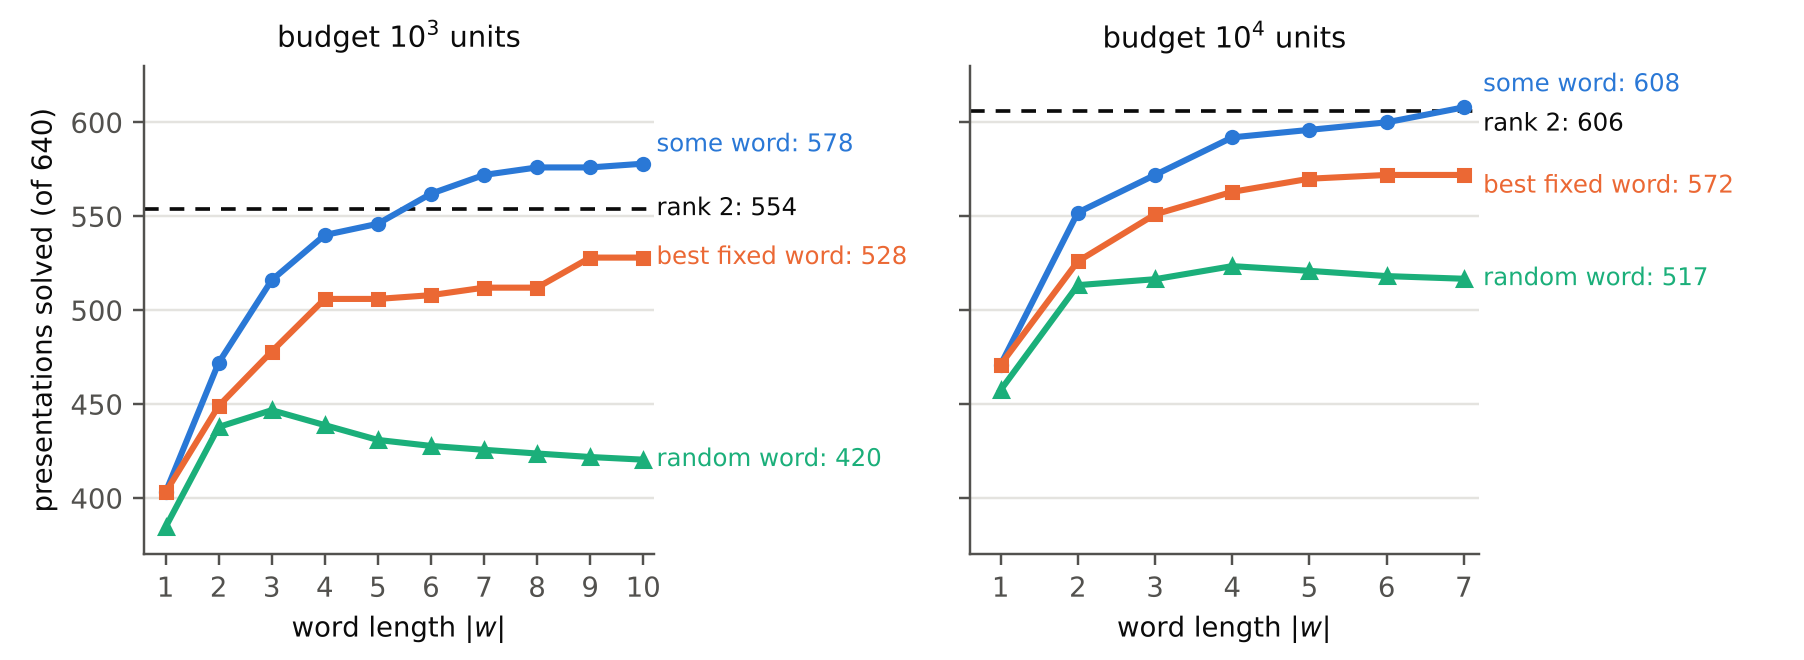
\includegraphics[width=\textwidth]{figures/stable_rank3_words.png}
\caption{Rank 3 against rank 2 on MS640. Some word and the best fixed word use the words of length at most $|w|$;
random word is $640$ times the share solved by the words of length exactly $|w|$. Dashed: rank 2.}
\label{fig:stable_words}
\end{figure}

\begin{table}[ht]
\centering
\small
\begin{tabular}{rrrrrrr}
\toprule
& & \multicolumn{2}{c}{words of length $|w|$} & \multicolumn{3}{c}{some word of length $\le|w|$}\\
\cmidrule(lr){3-4}\cmidrule(lr){5-7}
$|w|$ & words & solved & faster than rank 2 & solves & gained & lost\\
\midrule
1 & $2$ & $60.1\%$ & $0.0\%$ & $403$ & $0$ & $151$\\
2 & $6$ & $68.4\%$ & $1.1\%$ & $472$ & $0$ & $82$\\
3 & $18$ & $69.8\%$ & $0.6\%$ & $516$ & $0$ & $38$\\
4 & $54$ & $68.6\%$ & $1.1\%$ & $540$ & $4$ & $18$\\
5 & $162$ & $67.3\%$ & $0.9\%$ & $546$ & $8$ & $16$\\
6 & $486$ & $66.8\%$ & $0.7\%$ & $562$ & $16$ & $8$\\
7 & $1{,}458$ & $66.5\%$ & $0.6\%$ & $572$ & $20$ & $2$\\
8 & $4{,}374$ & $66.2\%$ & $0.6\%$ & $576$ & $22$ & $0$\\
9 & $13{,}122$ & $65.9\%$ & $0.5\%$ & $576$ & $22$ & $0$\\
10 & $39{,}366$ & $65.7\%$ & $0.5\%$ & $578$ & $24$ & $0$\\
\midrule
rank 2 & & $86.6\%$ & & $554$ & &\\
\bottomrule
\end{tabular}
\caption{Rank 3 at budget $10^3$. Solved: the share of the $640\times$words searches solved; faster: the share solved
in fewer units than rank 2, or solved where rank 2 fails. Gained: solved by some word, not by rank 2; lost: solved by
rank 2, by no word.}
\label{tab:stable_words}
\end{table}

\paragraph{Rank 3.} Rank 3 beats rank 2 only with the right word (Figure~\ref{fig:stable_words},
Table~\ref{tab:stable_words}). On the $554$ presentations rank 2 solves, a random word fails on $24.0\%$ and is
slower on $75.4\%$. The best fixed word, \texttt{yXYYYxyyy}, solves $528$. Some word passes rank 2 from length $6$
($578$ at length $10$; $608$ against $606$ at budget $10^4$), but finding it costs more than rank 2: trying the words
in shortlex order takes at least $41{,}711$ units on each of the $24$ gained, which rank 2 solves with $1{,}160$ to
$26{,}838$.

\paragraph{Why one letter costs more than one move.} With $w=x$, the relator $z^{-1}x$ lets one S-move turn a letter
$x^{\pm1}$ of another relator into $z^{\pm1}$, or back, without changing $\lambda$: $ux\cdot x^{-1}z=uz$. A state with
$m$ letters $x^{\pm1}$ thus has up to $2^m$ copies of the same length, all the same state once $z$ is set to $x$, and
the greedy pops them before any longer state. Over the $1{,}280$ searches with $|w|=1$, $97.5\%$ of the pops repeat a
state already popped, up to $z=x$. Where rank 2 solves and rank 3 fails, the $10^3$ pops reach a median of $12$
different states, while rank 2 needs a median of $116$ pops.


\paragraph{Ranks 4 and 5.} More generators are worse on every count (Table~\ref{tab:stable_ranks},
Figure~\ref{fig:stable_split}). Where rank 2 needs under $10$ units, almost every start solves but with more units;
the harder the presentation for rank 2, the more starts fail within the budget, and each added generator makes more
of them fail.

\subsection{One-shot change of variables}\label{sec:cov}

The naive stable search keeps $z$ and searches in rank $3$. A change of variables uses $z$ once, to remove $x$ or $y$,
and then searches in rank $2$ again.

\begin{definition}[Change of variables]\label{def:cov}
Let $P=\pres{x,y}{r_1,r_2}$ and let $w$ be a word in $x,y$ of length at least $2$.
\begin{enumerate}
  \item \emph{Stabilize}: $P_w=\pres{x,y,z}{r_1,\ r_2,\ z^{-1}w}$ (Definition~\ref{def:stab}).
  \item \emph{Substitute}: replace non-overlapping occurrences of $w^{\pm1}$ in $r_1,r_2$ by $z^{\pm1}$ and freely
  reduce. Call the results $r_1',r_2'$.
  \item \emph{Eliminate}: choose one of $r_1',r_2',z^{-1}w$ in which a generator $g\in\{x,y\}$ occurs exactly once.
  Write it cyclically as $g^{\epsilon}s$, with $g$ not in $s$, so that $g=s^{-\epsilon}$ in the group. Substitute
  $s^{-\epsilon}$ for $g$ in the other two relators and delete the chosen one.
\end{enumerate}
The result is a presentation $P'$ on the two generators $\{x,y,z\}\setminus\{g\}$, the \emph{image} of $P$. We rename
them $x,y$ and search $P'$ with LENGTH.
\end{definition}

\begin{example}
Let $P=\pres{x,y}{y^{-5}x^{-1}y^{4}x,\ y^{-2}xy^{-1}xy^{-1}x^{-1}}$ and $w=x^{-1}y$. Substituting $z$ for
$w$ ($3$ occurrences) gives
\[
P_w\ \to\ \pres{x,y,z}{y^{-5}zy^{3}x,\ \ y^{-1}z^{-2}y^{-1}x^{-1},\ \ z^{-1}x^{-1}y}.
\]
In the first relator $x$ occurs once: $x=y^{-3}z^{-1}y^{5}$. Substituting it into the other two and renaming
$y,z$ as $x,y$ gives the image
\[
P'=\pres{x,y}{x^{-1}y^{-2}x^{-6}yx^{3},\ \ y^{-1}x^{-5}yx^{4}}.
\]
\end{example}

\begin{definition}[One-shot CoV]\label{def:oneshot}
The words $w$ are the cyclic subwords of $r_1$ and $r_2$ of length at least $2$, one of each pair $\{w,w^{-1}\}$,
except those whose substitution leaves a relator with fewer than $3$ letters. Step 2 substitutes every
non-overlapping occurrence, read left to right; step 3 tries $g=x$ and $g=y$ and every relator in which $g$ occurs once.
Each choice gives one image, and the images are ordered by $|w|$, then by $w$. The one-shot policy runs LENGTH with
$10^3$ units on $P$ itself, then on the images in this order, $10^3$ units each, and stops at the first solve or after
$10^4$ units in total. $P$ is searched at cap $24$, an image at cap $\max(24,\ \text{longest relator of }P'+16)$.
\end{definition}

On MS640 a presentation has $8$ to $174$ images (median $56$). The policy reaches at most the first $9$ of them, since
$P$ takes the first $10^3$ units.

\paragraph{Score.} Table~\ref{tab:cov_oneshot} compares the policy with LENGTH on $P$ at the same total budget of
$10^4$ units. Every solve was replayed: an AC path on $P$, a stable certificate by redoing the change of variables and
then the path on $P'$.

\begin{table}[ht]
\centering
\small
\begin{tabular}{lrrrrrr}
\toprule
& & \multicolumn{2}{c}{AC path of $P$} & & & LENGTH\\
\cmidrule(lr){3-4}
benchmark & solved & from $P$ & from $\varphi(P)$ & stable certificate & units spent & at $10^4$\\
\midrule
MS640 & $584$ & $554$ & $0$ & $30$ & $693{,}162$ & $606$\\
bench60 & $39$ & $29$ & $0$ & $10$ & $246{,}744$ & $40$\\
ladder100 & $46$ & $11$ & $13$ & $22$ & $734{,}766$ & $20$\\
\bottomrule
\end{tabular}
\caption{One-shot CoV, $10^3$ units per search and $10^4$ per presentation. Units spent: summed over the benchmark,
failures included.}
\label{tab:cov_oneshot}
\end{table}

\begin{table}[ht]
\centering
\small
\begin{tabular}{llrrrr}
\toprule
& & \multicolumn{2}{c}{units to solve} & \multicolumn{2}{c}{S-moves}\\
\cmidrule(lr){3-4}\cmidrule(lr){5-6}
benchmark & solved by & median & max & median & max\\
\midrule
MS640 & $P$ & $9$ & $990$ & $8$ & $101$\\
& image & $2{,}400$ & $9{,}840$ & $49.5$ & $100$\\
bench60 & $P$ & $61$ & $875$ & $16$ & $47$\\
& image & $1{,}556.5$ & $9{,}840$ & $45.5$ & $69$\\
ladder100 & $P$ & $4{,}092.5$ & $9{,}833$ & $31$ & $113$\\
& image & $5{,}138.5$ & $8{,}963$ & $43$ & $120$\\
\bottomrule
\end{tabular}
\caption{The solves of Table~\ref{tab:cov_oneshot}. Units to solve count every unit of the presentation, the search on
$P$ included. S-moves are those of the solving search, on $P$ or on $P'$; for ladder100, solved by $P$ includes the
$13$ solves through $\varphi(P)$.}
\label{tab:cov_oneshot_cost}
\end{table}

On MS640 and bench60 every AC path comes from the search on $P$ within its first $10^3$ units: the images add only
stable certificates, $30$ and $10$. LENGTH spends the same remaining $9\times10^3$ units on $P$ and gains more, $52$
and $11$. On ladder100 the order is reversed, $46$ against $20$: its rows are graded by the units LENGTH needs
(Definition~\ref{def:ladder}), so LENGTH alone is weak there by construction. On MS640 the solving image is one of the
first $9$, and the first in $15$ of the $30$; its word is $x^{-1}y$ ($14$), $yx$ ($7$), $xy$ ($7$) or $x^{-1}y^{2}$
($2$).

\paragraph{Every image.} The one-shot policy sees a few images. To see what the images can do at all, we searched every
image of every MS640 presentation, each with the full budget. This family is larger: $w$ is any cyclic subword of
length $2$ to $|r_i|-1$, every set of non-overlapping occurrences is substituted, and images equal up to relator order,
rotation, inversion and the $8$ signed permutations of $x,y$ are searched once. That gives $114{,}042$ images, $5$ to
$10{,}740$ per presentation (median $36$), $335$ CPU-hours in all. The \emph{best image} counts a presentation as
solved if some image of it is solved; like some word in Section~\ref{sec:stable}, it needs the right image in advance
and is a bound, not a method.

\begin{table}[ht]
\centering
\small
\begin{tabular}{rrrrrr}
\toprule
budget & & best & & random image & units to search\\
per search & LENGTH on $P$ & image & gained & solves & every image\\
\midrule
$10^2$ & $455$ & $555$ & $100$ & $67.3\%$ & $5{,}328$\\
$10^3$ & $554$ & $604$ & $50$ & $82.3\%$ & $28{,}456$\\
$10^4$ & $606$ & $626$ & $20$ & $90.8\%$ & $164{,}759$\\
$10^5$ & $634$ & $640$ & $6$ & $95.8\%$ & $657{,}198$\\
\bottomrule
\end{tabular}
\caption{Every image on MS640. Gained: solved by the best image, not by LENGTH on $P$; no presentation is lost.
Random image: the share of a presentation's images that are solved, averaged over the $640$ presentations. Units to
search every image: the mean over presentations, a failed search counted at the full budget.}
\label{tab:cov_all}
\end{table}

The best image passes LENGTH at every budget, but the margin falls from $100$ to $6$, and finding the image costs more
than the margin (Table~\ref{tab:cov_all}). At $10^3$, searching every image takes a mean of $28{,}456$ units per
presentation, against $10^4$ for LENGTH to reach $606$. A random image is worse than $P$: at $10^4$ it needs fewer units
than $P$ in $33.0\%$ of the pairs, the same in $9.6\%$, more in $48.2\%$, and fails in $9.2\%$. On the $606$
presentations both solve at $10^4$, the best image needs a mean of $86$ units and $12.8$ S-moves, against $390$ units
and $20.0$ S-moves for $P$. Images run at a cap of $24$ to $91$ and $P$ at $24$, so the comparison favours the images.

\begin{figure}[ht]
\centering
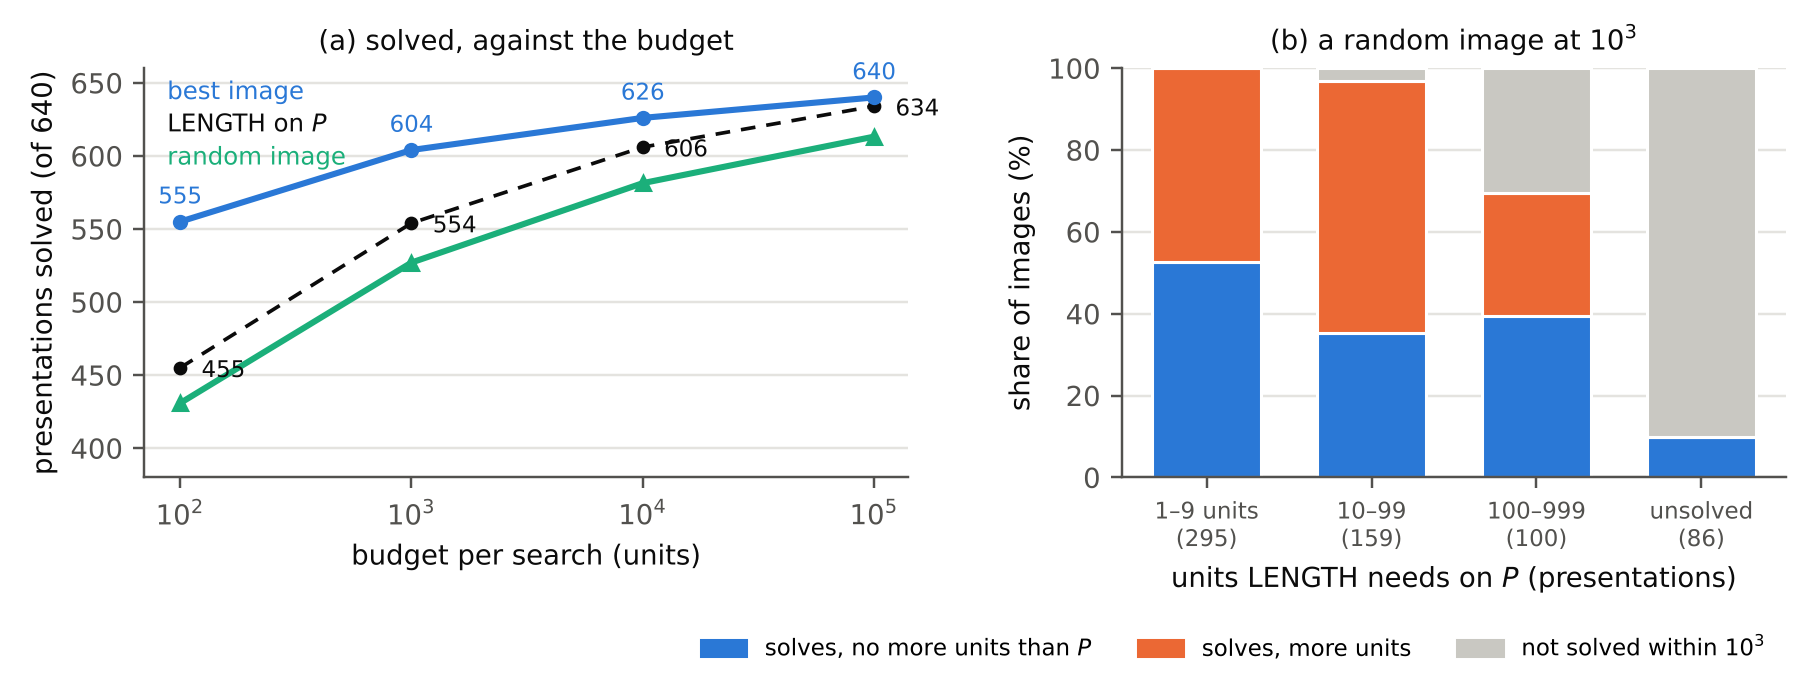
\includegraphics[width=\textwidth]{figures/cov_images.png}
\caption{Every image on MS640. (a) Presentations solved by LENGTH on $P$, by the best image, and by a random image
($640$ times the mean share of a presentation's images solved). (b) A random image against LENGTH on $P$ at budget
$10^3$, with MS640 grouped by the units LENGTH needs on $P$; compare Figure~\ref{fig:stable_split}.}
\label{fig:cov_images}
\end{figure}

The best image passes LENGTH at every budget, but the margin falls from $100$ to $6$, and finding the image costs more
than the margin (Table~\ref{tab:cov_all}, Figure~\ref{fig:cov_images}a). Unlike a stable start, an image is often
cheaper than $P$ (Figure~\ref{fig:cov_images}b): where LENGTH needs $1$ to $9$ units, $52.6\%$ of the images solve in
no more units, and where LENGTH fails within $10^3$, $9.8\%$ of the images still solve.

\paragraph{The best image, then LENGTH.} Search each presentation from its best image only. Then LENGTH solves all
$640$ presentations of MS640 within $14{,}473$ units each, $295{,}268$ units in all (mean $461$, median $7$), with
paths of median $6$ and at most $489$ S-moves. LENGTH on $P$ still misses $6$ at $10^5$ units.
\begin{center}
\small
\begin{tabular}{lrrrrrr}
\toprule
budget (units) & $10$ & $10^2$ & $10^3$ & $10^4$ & $3\cdot10^4$ & $10^5$\\
\midrule
best image, then LENGTH & $416$ & $555$ & $604$ & $626$ & $640$ & $640$\\
LENGTH on $P$ & $317$ & $455$ & $554$ & $606$ & $626$ & $634$\\
\bottomrule
\end{tabular}
\end{center}
The last $36$ presentations are the rows with $n=7$, $r_1=y^{-8}x^{-1}y^{7}x$; their best images need about
$14{,}400$ units and give paths of $489$ S-moves. The best image is chosen with hindsight: finding it by searching every
image costs a mean of $657{,}198$ units per presentation at budget $10^5$.


% ---- Appendix: details moved out of the main text ----
\appendix
\section{bench60}\label{app:bench60}

\begin{definition}[bench60, full rule]\label{def:bench60full}
Let $g_0=3$ and $g_{10}=574{,}959$ be the least and the largest value of $g$ on MS640 at budget $10^6$, and
let $\rho=(g_{10}/g_0)^{1/10}\approx3.37$. \emph{Bin} $b\in\{0,\dots,9\}$ is the set of $P\in$ MS640 with
$g_0\rho^{b}\le g(P)<g_0\rho^{b+1}$ (bin $9$ closed on the right). \textbf{bench60} takes $6$ presentations from every
bin by the following rule.
\begin{enumerate}
  \item Over the whole subset, minimise the number of pairs of chosen presentations in the same $\Aut(\F_2)$-orbit.
  \item Subject to (1), sort the presentations of each bin by path length, the number of S-moves in the solution GS-SUB finds; break ties by smaller $g$ first, then by line number in MS640.
  Take the $6$ presentations closest to $6$ evenly spaced positions of this sorted list, the first and the last
  position included.
  % This one needs more explaination
\end{enumerate}
\end{definition}

Figure~\ref{fig:bench60} shows where the $60$ rows lie in MS640.

\begin{center}
\begin{tabular}{rrrrr}
\toprule
bin $b$ & range of $g$ & rows of MS640 & rows of bench60 & mean $g$ on bench60\\
\midrule
0 & $[3,\,11)$ & $317$ & $6$ & $6.3$\\
1 & $[11,\,35)$ & $89$ & $6$ & $17.7$\\
2 & $[35,\,116)$ & $63$ & $6$ & $74.3$\\
3 & $[116,\,390)$ & $60$ & $6$ & $261.7$\\
4 & $[390,\,1{,}314)$ & $31$ & $6$ & $691.2$\\
5 & $[1{,}314,\,4{,}433)$ & $26$ & $6$ & $1{,}746.8$\\
6 & $[4{,}433,\,14{,}959)$ & $28$ & $6$ & $9{,}869.2$\\
7 & $[14{,}959,\,50{,}482)$ & $14$ & $6$ & $19{,}596.3$\\
8 & $[50{,}482,\,170{,}367)$ & $6$ & $6$ & $66{,}530.7$\\
9 & $[170{,}367,\,574{,}959]$ & $6$ & $6$ & $353{,}647.7$\\
\midrule
all & & $640$ & $60$ & \\
\bottomrule
\end{tabular}
\end{center}

\begin{figure}[ht]
\centering
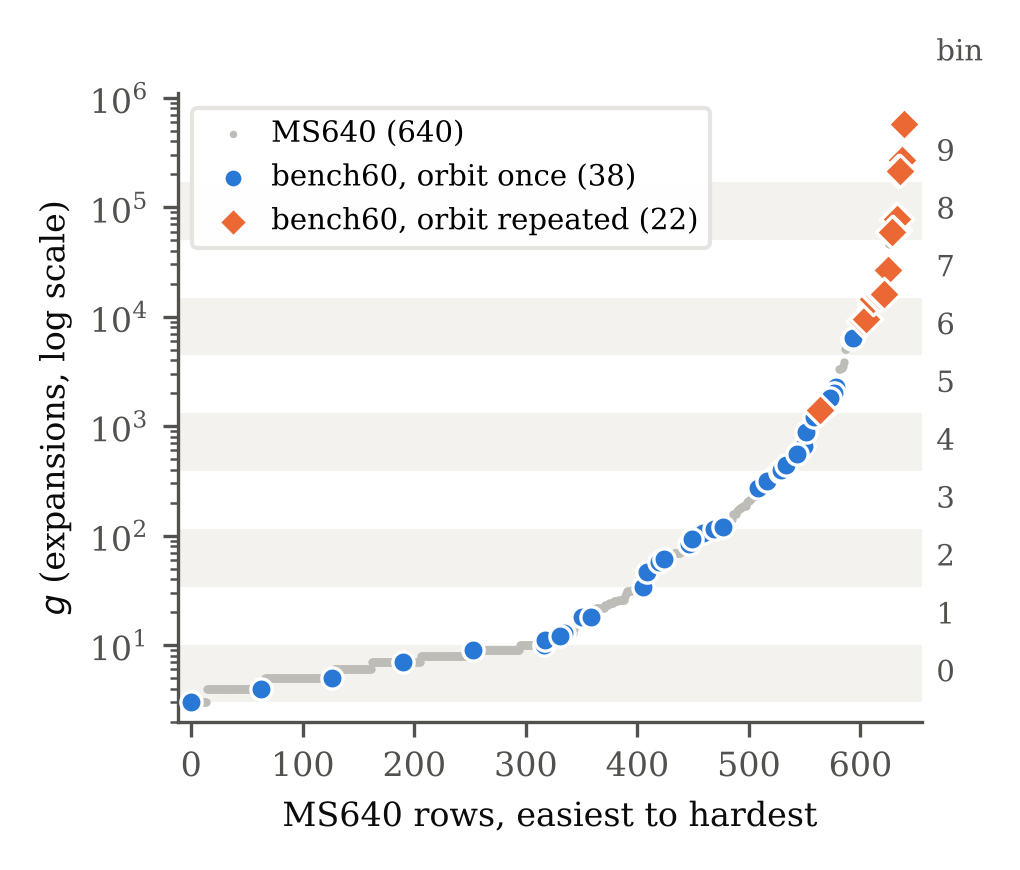
\includegraphics[width=0.49\textwidth]{figures/bench60_g.png}\hfill
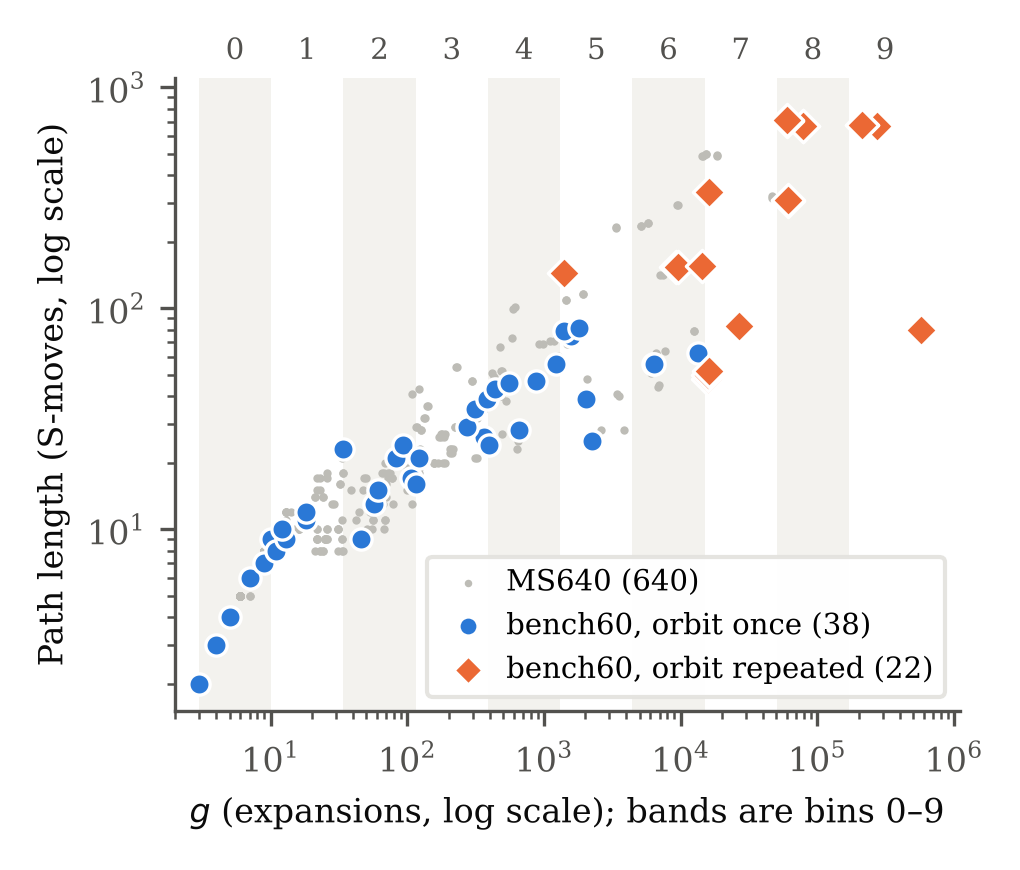
\includegraphics[width=0.49\textwidth]{figures/bench60_path.png}
\caption{bench60 inside MS640. Grey: all $640$ presentations; colour: the $60$ choices, six per bin. Blue circles are choices whose
$\Aut(\F_2)$-orbit occurs once in bench60; diamonds are choices that share an orbit with another choice, which bins 7--9 force.
Left: $g$ against the rows sorted by $g$; the shaded bands are bins 0--9, each $3.37$ times the one below.
Right: the S-move length of a presentation against $g$.}
\label{fig:bench60}
\end{figure}


\begin{thebibliography}{9}
\bibitem{SMM24} A.~Shehper, A.~M.~Medina-Mardones, L.~Fagan, B.~Lewandowski, A.~Gruen, Y.~Qiu, P.~Kucharski,
Z.~Wang and S.~Gukov, \emph{What makes math problems hard for reinforcement learning: a case study}, arXiv:2408.15332,
2024.
\bibitem{FTS26} L.~Fagan, M.~Tarquini, A.~Shehper, M.~Manko, A.~Gruen, C.~Huang, G.~Butbaia, D.~Passaro and
S.~Gukov, \emph{The Two-Hump Problem: Bridging the Difficulty Gap in Mathematical Reinforcement Learning}, Proceedings
of the 43rd International Conference on Machine Learning (ICML), 2026, arXiv:2606.21611.
\end{thebibliography}


\end{document}
